\begin{figure}[!htbp]
\centering
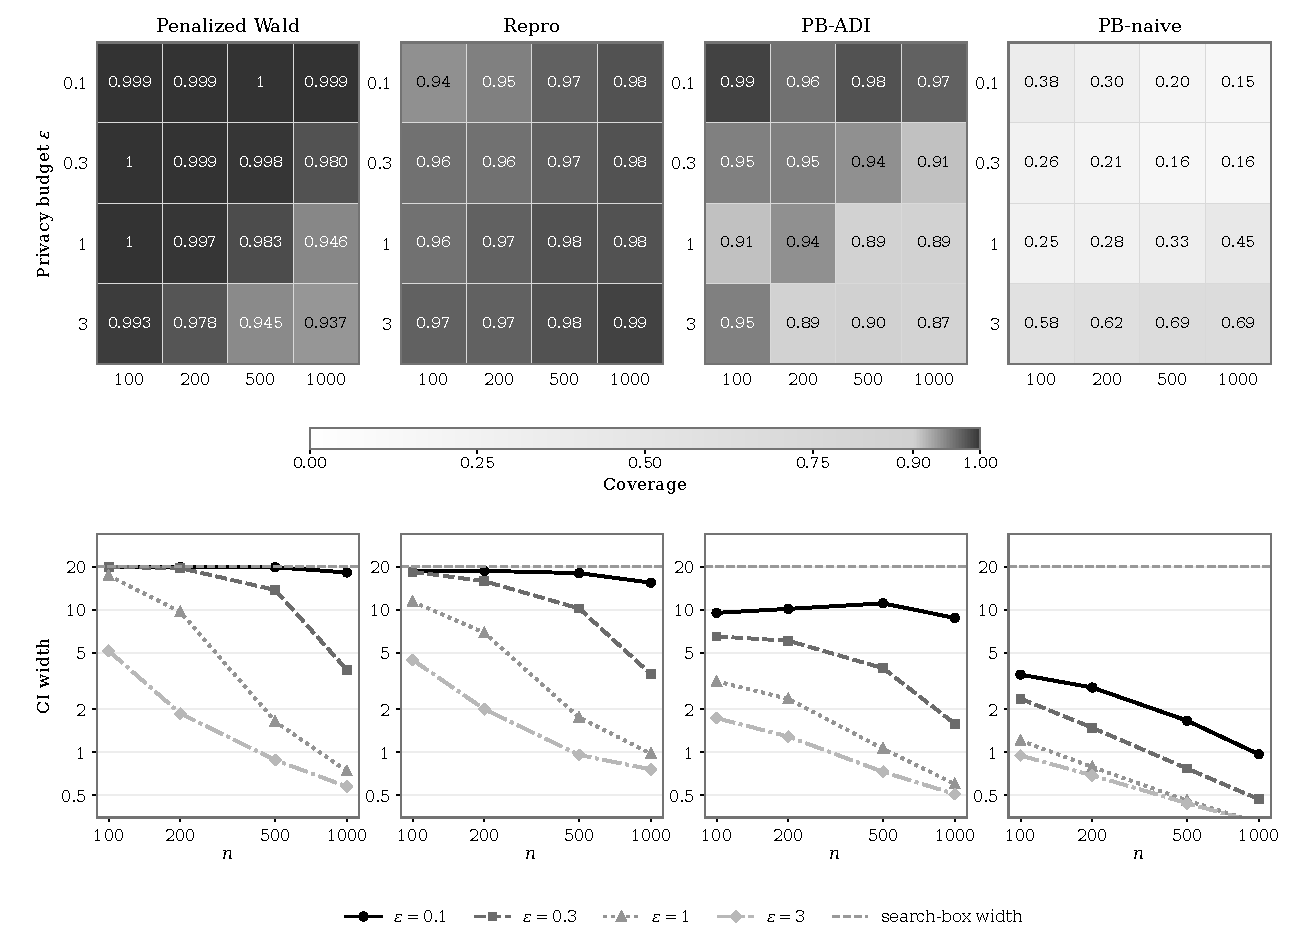
\includegraphics[width=0.98\linewidth]{results/figures/fig_exp3_comparison.pdf}
\caption{Experiment 3. Coverage of the $90\%$ interval for $\beta_1^\ast$ (first row) and its average width (second row), over $1000$ replications per cell. In the heat maps the rows are the privacy budget and the columns the sample size; the grey scale breaks at the nominal level $0.90$, so cells below it are light, and the finite-$R$ coverage bound is $0.90050$. In the width panels the dashed line marks the total width $20$ of the search region $[-10,10]$: an interval approaching it is box-limited and therefore uninformative about efficiency, and we draw no comparison from such a cell. This is a property of the interval and not of the numerical search, which does not substitute the search region when it fails to resolve. Comparison values are those reported by Wang, Chang and Awan (2026, Fig.~6), whose figure and caption state $90\%$ intervals.}
\label{fig:exp3-comparison}
\end{figure}
